\chapter{System Description}\label{chap:systemDescribtion}
The overall idea of the project is to consider several satellites flying in formation, with an agnle in between and with the purpose of maintaining the angle by using the drag force. As a proof of concept, an AAU-CubeSat will be used, by choosing eight AAU-CubeSat that orbits the Earth as shown in  \figref{fig:1}. In this project, all CubeSat's will be assumed identical. Moreover, a full-scale implementation of the system will not be possible, therefore, the whole system will be simulated using MATLAB and Simulink. 
%
\begin{figure}[H]
	\centering
	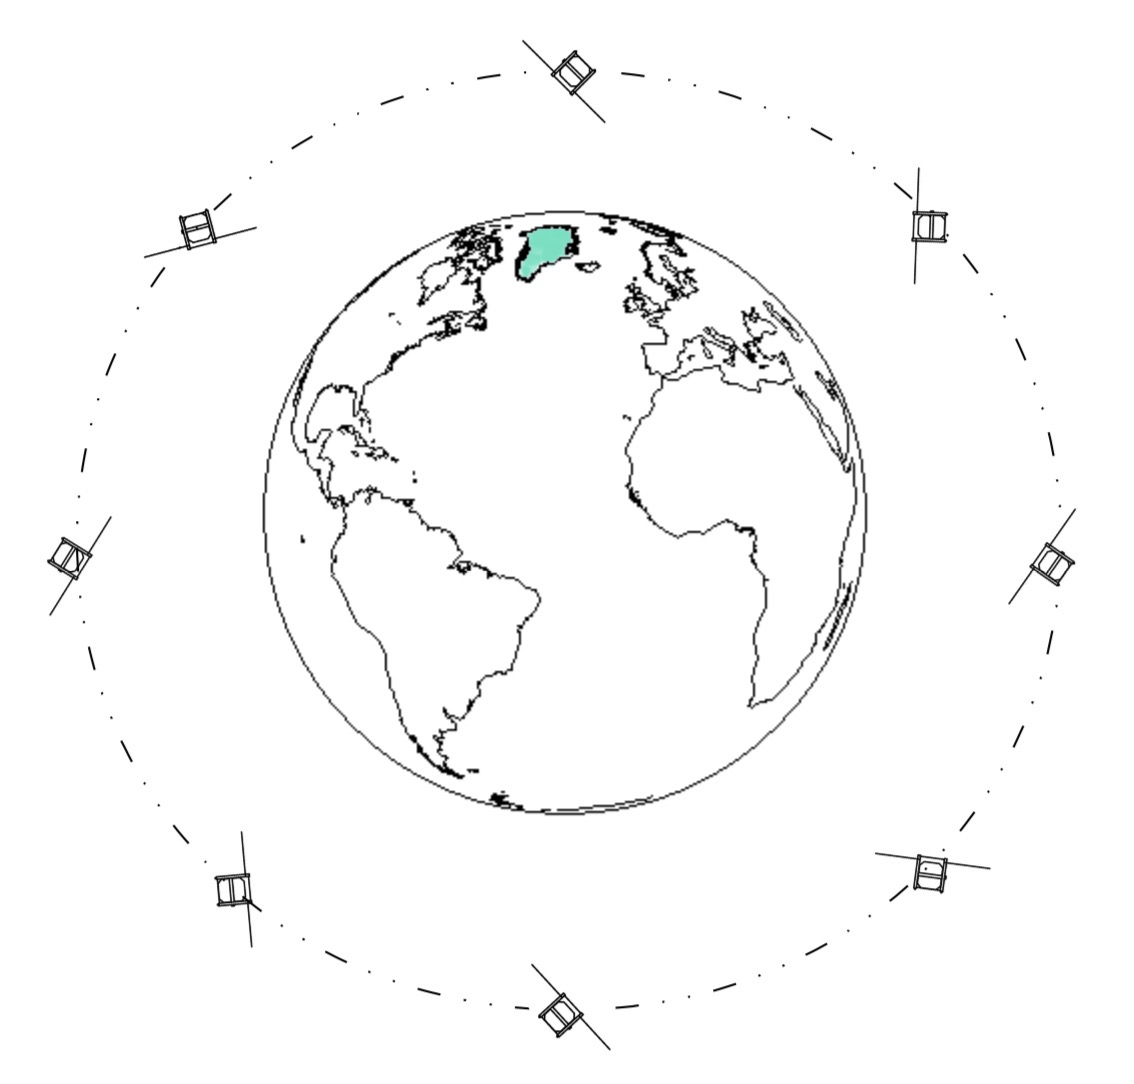
\includegraphics[width=0.7\linewidth]{figures/sat_form}
	\caption{Eight satellites in flying formation on orbit}
	\label{fig:1}
\end{figure}
%
\section{About AAU-CubeSat}
The AAU-CubeSat shown in \figref{fig:pico} is a pico-satellite developed by Stanford University,  assembled at Aalborg University by students and used mainly for Low Earth Orbit (LEO)  tests.
\begin{figure}[H]
	\centering
	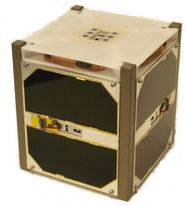
\includegraphics[width=0.3\linewidth]{figures/cub}
	\caption{View of CubeSat satellite \cite{cs}}
	\label{fig:pico}
\end{figure}
The pico-satellite is designed for LEO, therefore a few constraints are imposed. The CubeSat is limited in size and weight. The dimensions of the satellite are $10cm\times10cm\times10cm$, while the weight is around 1 kg.\cite{CDS}

In order to place the CubeSat on orbit, a deployment system is used, called P-POD. This system uses the force of a spring to launch the satellite into space. The satellite will be placed inside the launch rocket as payload. By using this system, an important advantage is reducing the cost of the launch. \cite{PPOD}
%
\section{AAU-CubeSat actuators}
The selection of attitude control components is important in order to meet the performance requirements. For this project, three magnetorquers and three momentum wheels have been chosen as actuators. Initially, using only three momentum wheels has been considered, but the downside of using only momentum wheels is that some amount of momentum can be stored in the wheels, which will imply having a way to take back all that momentum. Therefore, a way get rid of saturation in the wheels is to use an external torques (magnetorquers). 

\textbf{Magnetorquers} are wire coils which generate an electromagnetic field. The field interacts with the Earth magnetic field and a torque is generated for stabilizing the satellite. An important aspect of the magnetorquer is when a reaction wheel reaches a maximum speed and can no longer produce the torque this is referred as wheel saturation, so a magnetorquer is used to extract the momentum from the wheel.
%
\begin{table}[H]
	\begin{minipage}[b]{0.49\linewidth}
		\centering
		\begin{figure}[H]
			\centering
			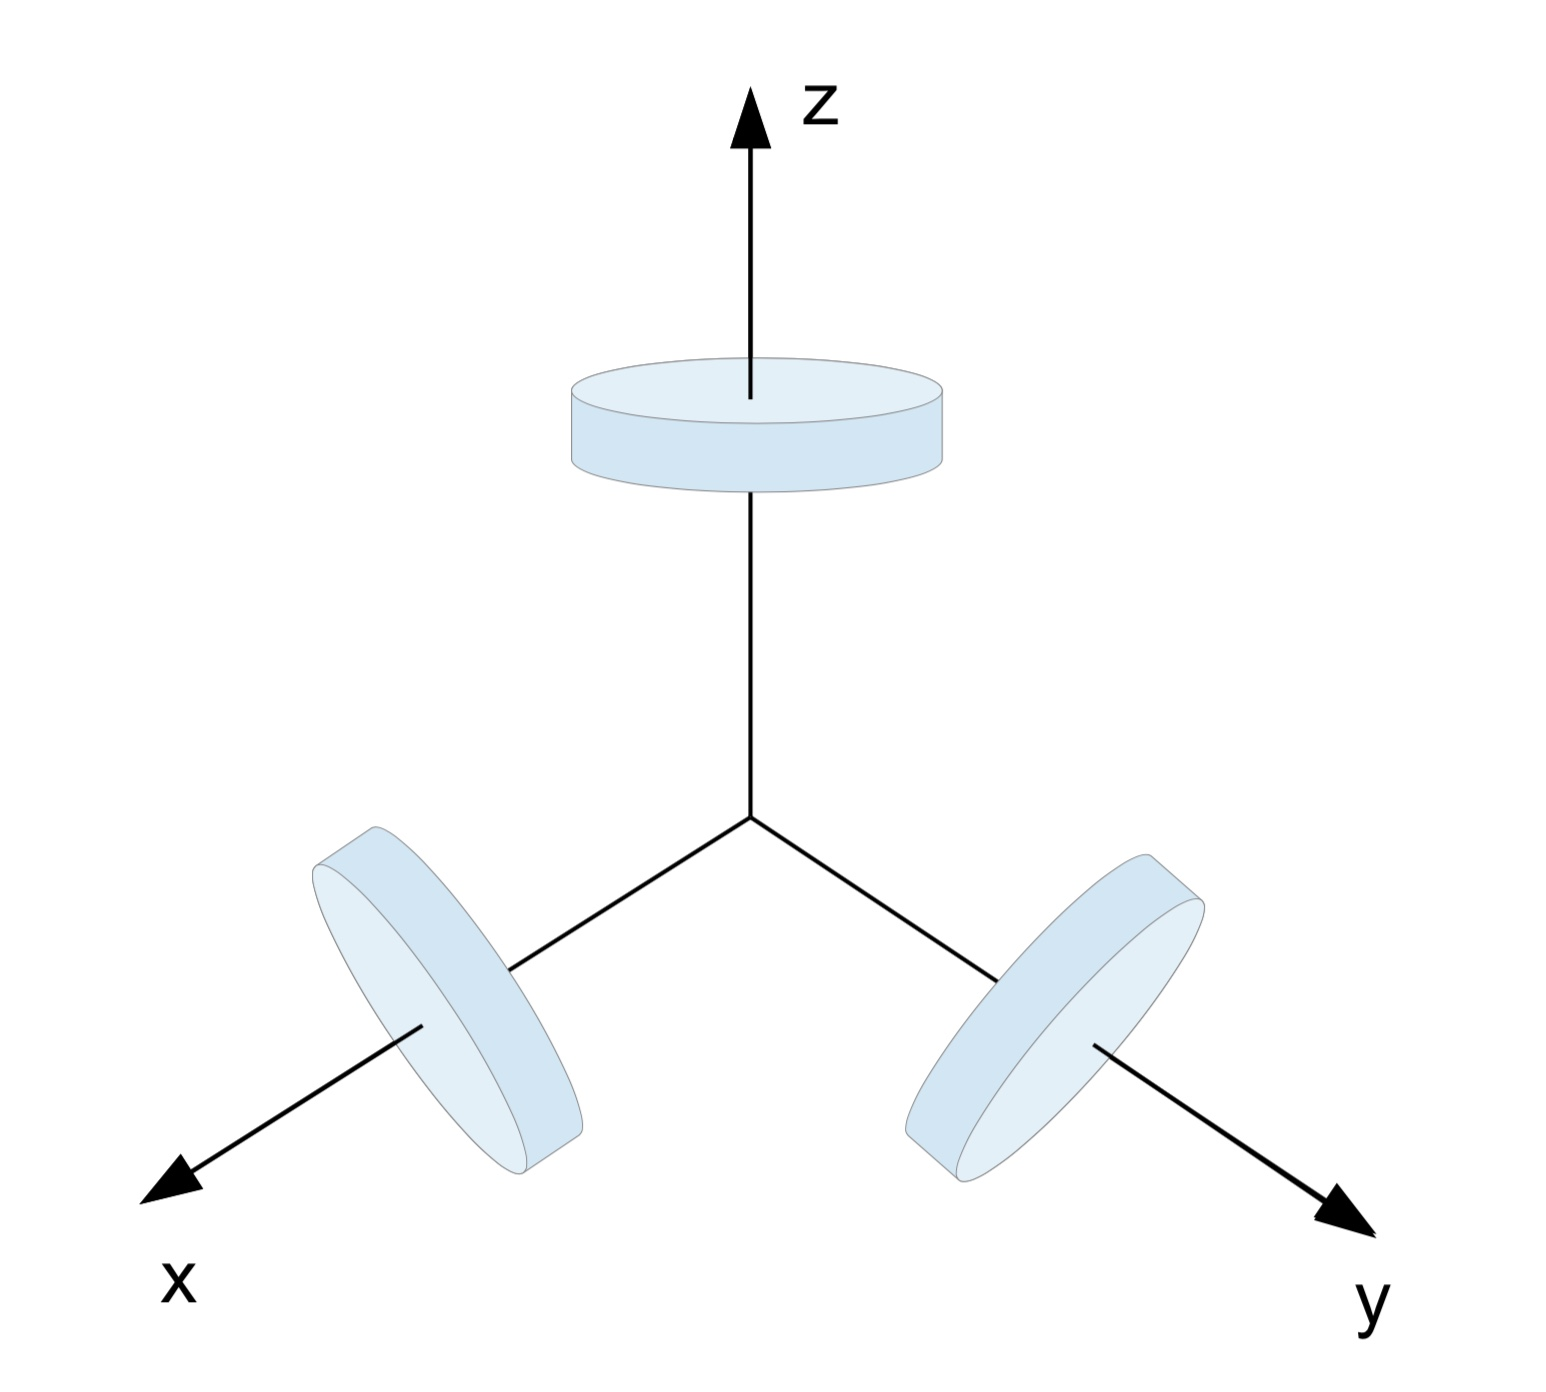
\includegraphics[width=0.9\linewidth]{figures/RW}
			\caption{Example of three reaction wheel for CubeSat}
			\label{fig:MW}
		\end{figure}
	\end{minipage}\hfill
	\begin{minipage}[b]{0.49\linewidth}
		\centering
		\begin{figure}[H]
			\centering
			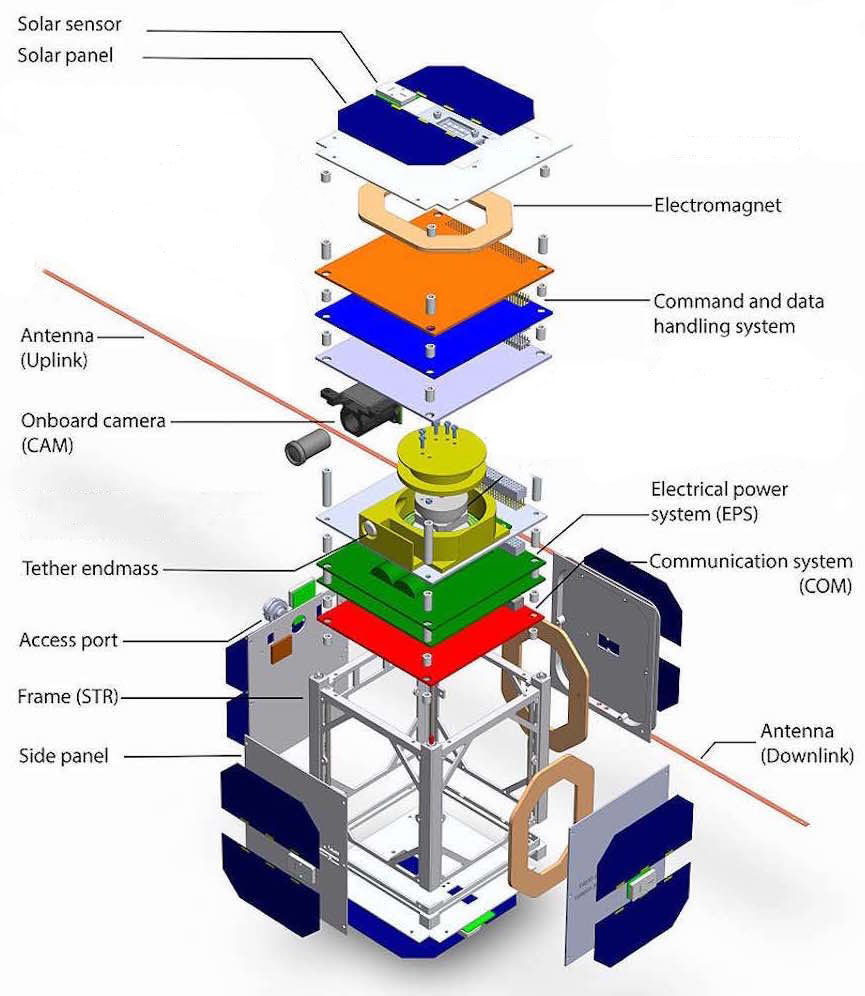
\includegraphics[width=1\linewidth]{figures/cubsat1}
			\caption{Expanded view for CubeSat \cite{view}}
			\label{fig:csat}
		\end{figure}
	\end{minipage}
\end{table}
%
\textbf{Reaction wheels} shown in \figref{fig:MW} strength is that no information is needed about the magnetic field in order to control the CubeSat torque. These wheels are capable to store the momentum needed for maneuvering or pointing.
% Removing energy from the system it can be proved easily by using the drag force, but gaining energy it might be possible if thrusters are used.
%  colloid thruster or "electrospray thruster"
\section{AAU-CubeSat sensors}
The CubeSat can sustain itself using solar pannels. In the middle of solar panels, a sun sensor similar in \figref{fig:csat} provides a vector equal to the direction of the sun and also a vector of the Earth's magnetic field measured by the magnetometer. Whether the Earth’s magnetic field is measured, or the sun vector, the objective is to use these sensors to deliver vector solutions for determining the satellite’s orientation and rotation rates.

\textbf{Magnetometer} is a sensor used for attitude control, which measure the direction and intensity of the magnetic field. The atittude is determined from the magnetometer by comparing the measure magnetic field with a referance field.

\textbf{Sun sensor} is used for estimating the position of the Sun and delivering a vector of measurements from the Sun.
\section{Coordinate frames}
In order to determine the attitude in three-dimensional space, three different coordinate frames are defined.
\begin{figure}[H]
	\centering
	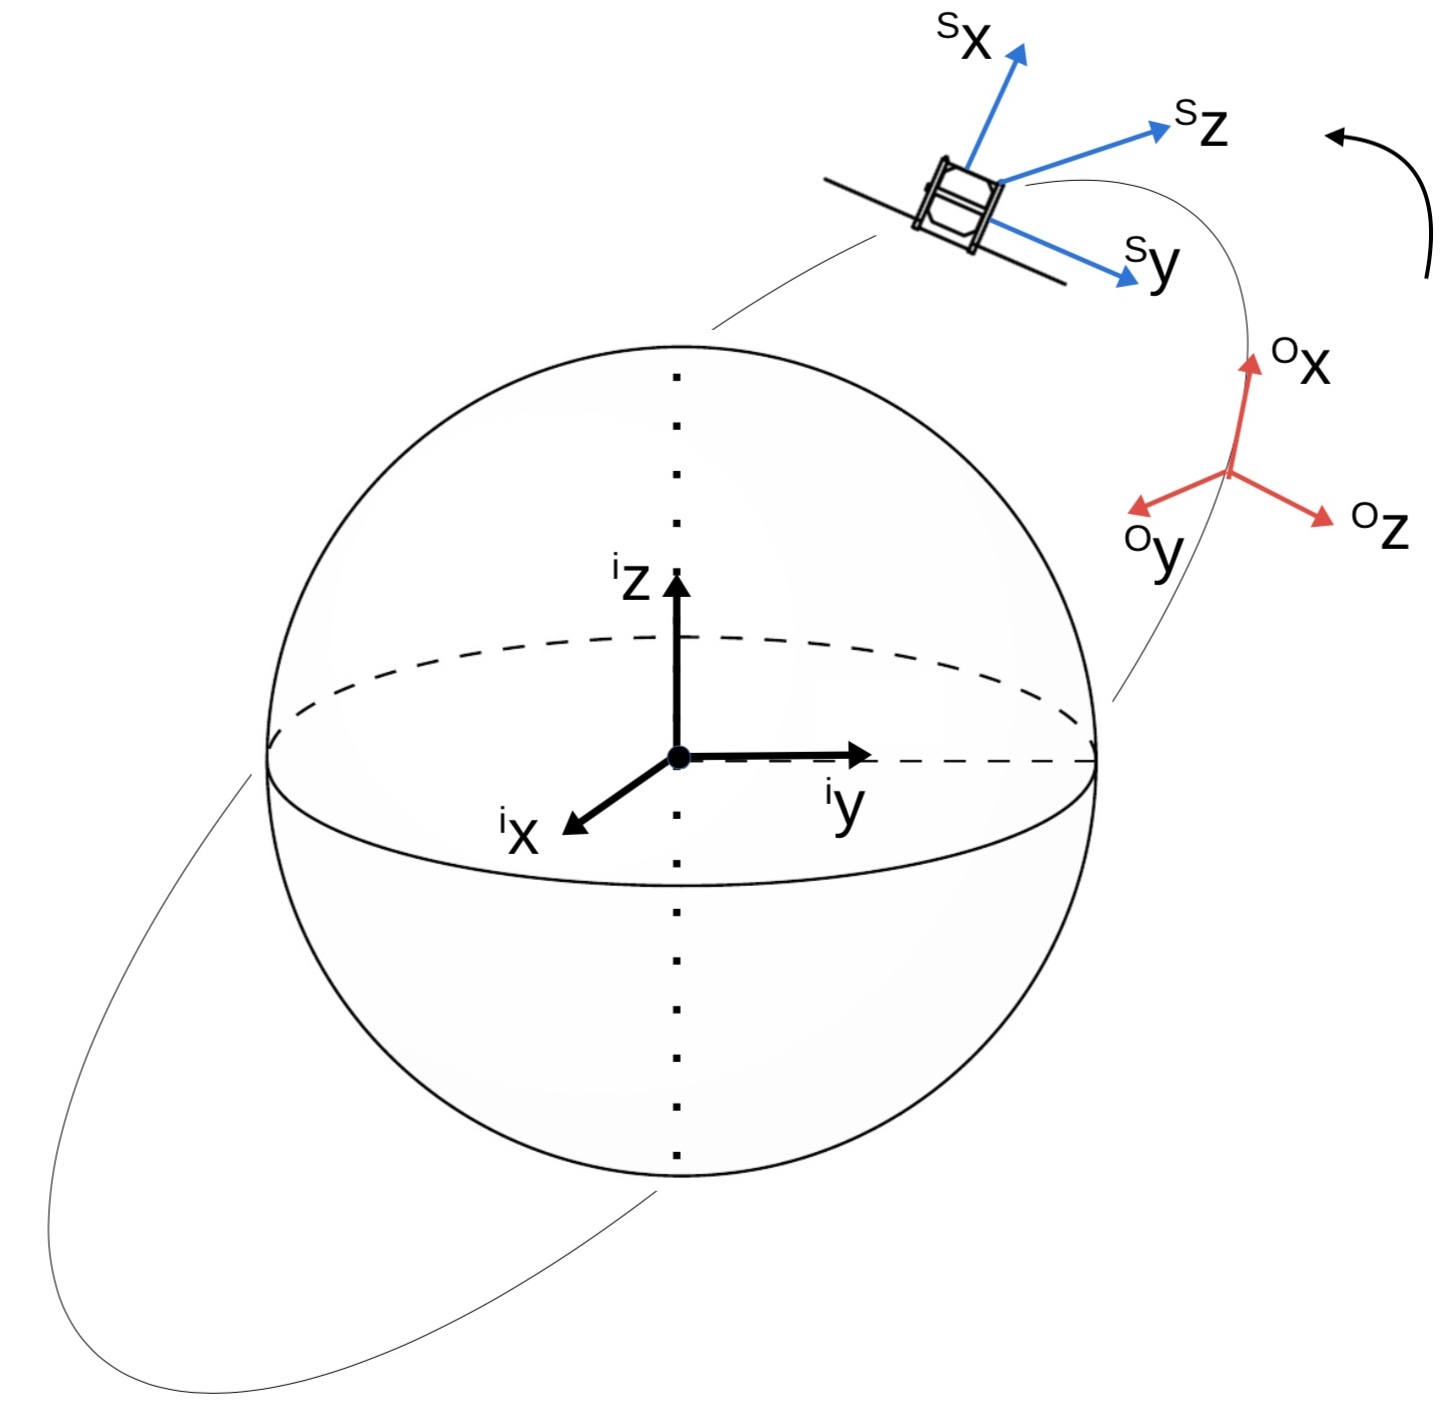
\includegraphics[width=0.7\linewidth]{figures/ref_frames}
	\caption{Representation of the three coordinate frames }
	\label{fig:ref_frames}
\end{figure}
\subsubsection{\textit{Earth Centered Inertial frame(ECI)}}
The equations of motion that describe the formation satellite are used in the ECI frame shown in \figref{fig:ref_frames}, since it can be seen as a non-accelerating frame. The $^iz$ axis is pointing through the geographical north pole, the $^ix$ axis is crossing from the point where the equatorial of the earth and the vernal equinox met and the $^iy$ axis is the cross product of $^ix$ and $^iz$ creating a right-handed coordinate system. 
\subsubsection{\textit{Orbit Reference frame(ORF)}}
The orbit reference shown in \figref{fig:ref_frames} is placed in the center of the satellite and defined with the $^oy$ axis always pointing at the Nadir point, the $^ox$ axis is tagent to the orbit in the direction of the satellite velocity and $^oz$ is the cross product of the $^ox$  and $^oy$. 
\subsubsection{\textit{Satellite Body Frame(SBF)}}
The satellite body frame is placed in the center of mass of the satellite as shown in  \figref{fig:ref_frames} and the axis are defined as represented in \figref{fig:refframes} and rotating with the satellite.
\begin{figure}[H]
\centering
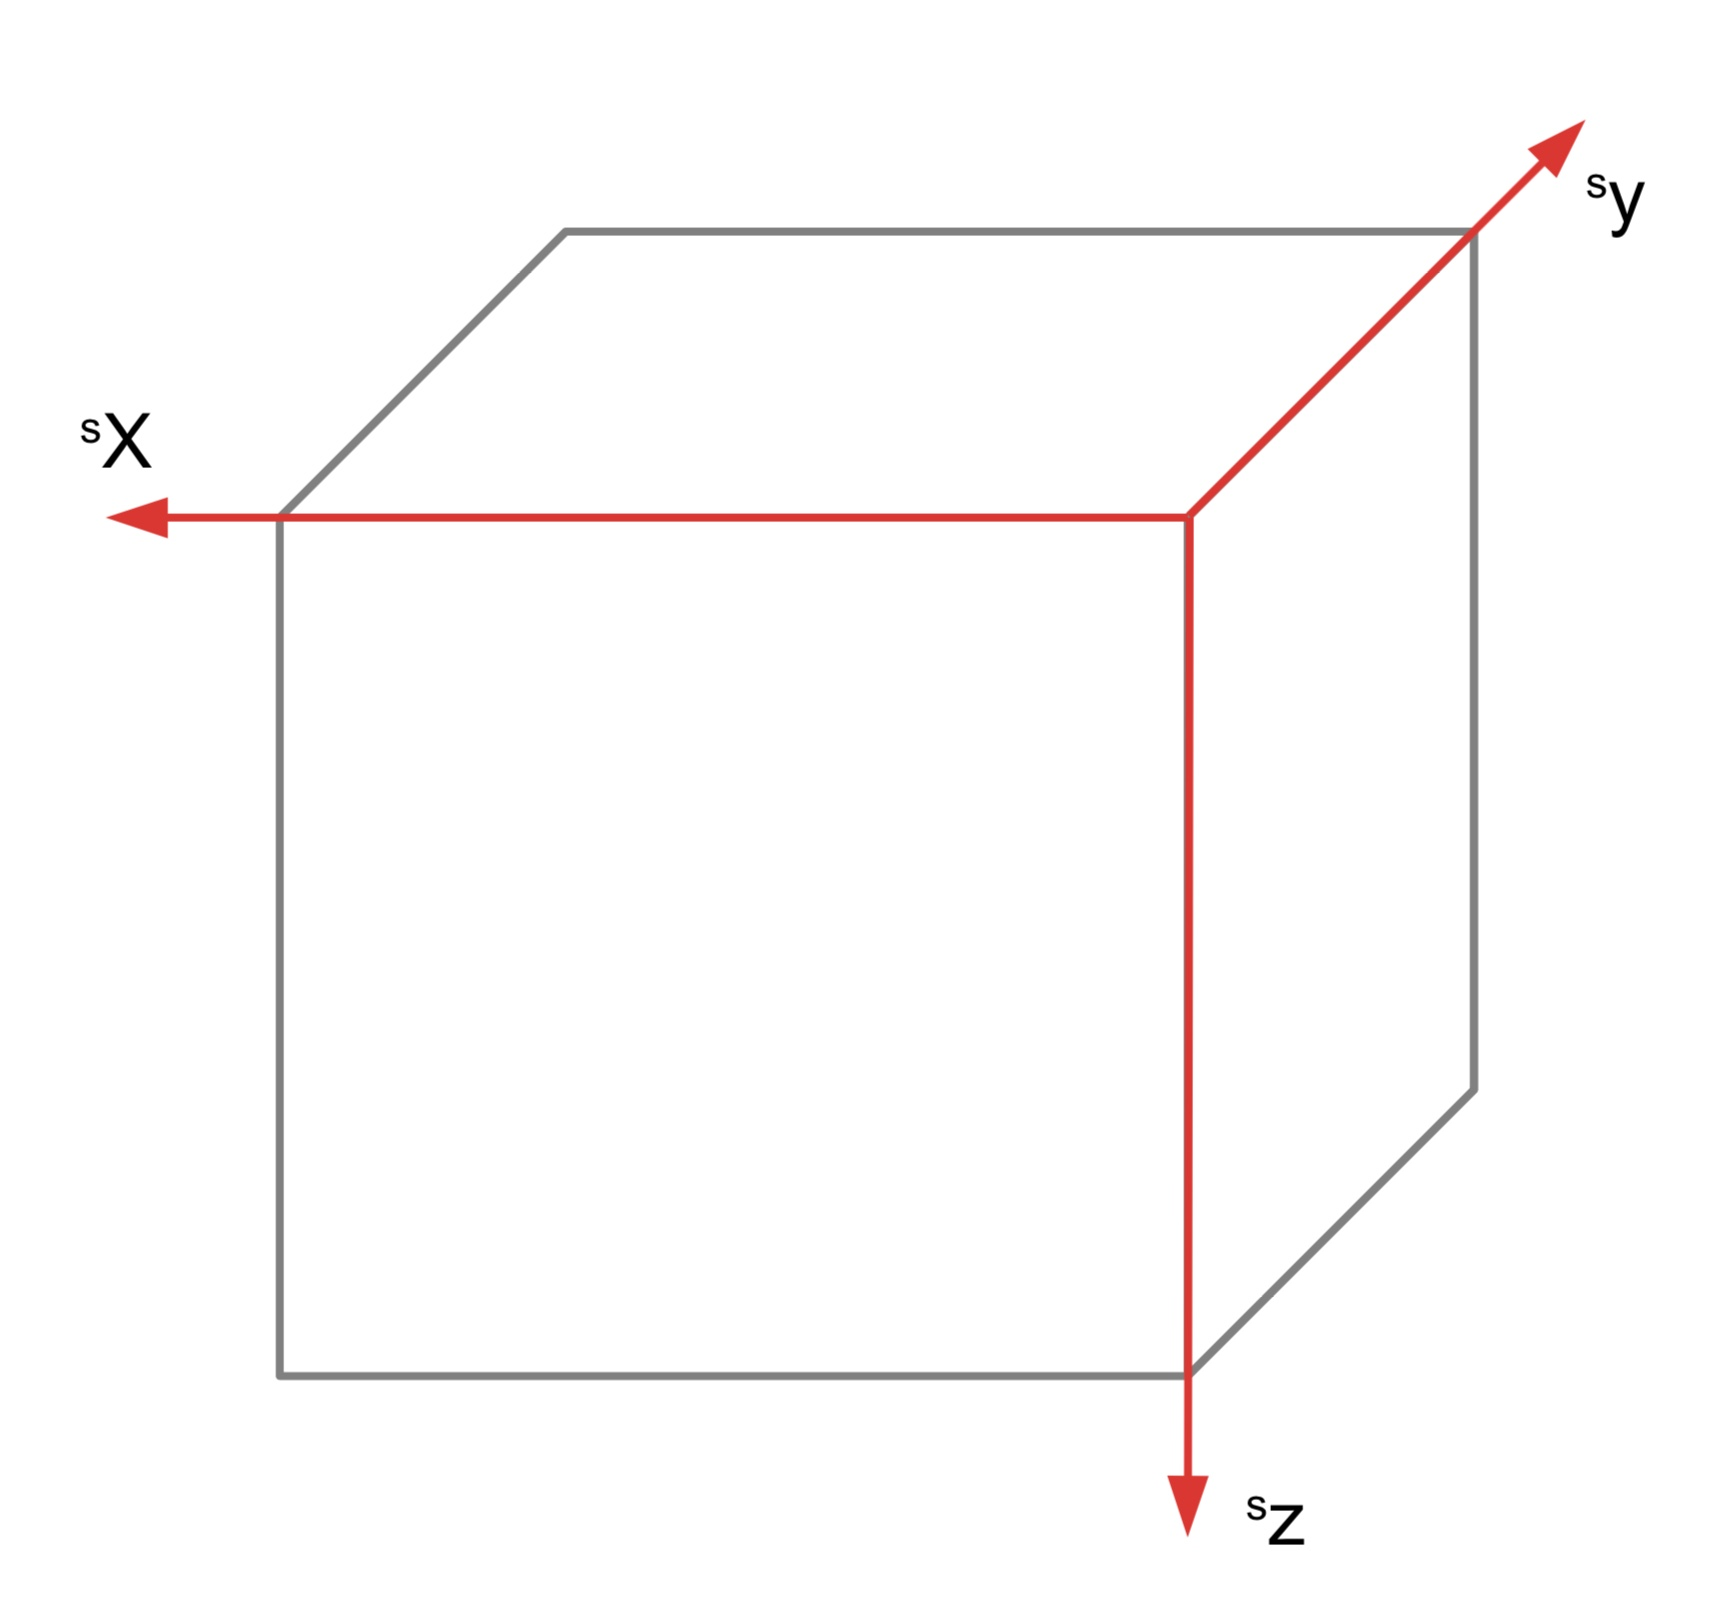
\includegraphics[width=0.5\linewidth]{figures/frames}
\caption{Satellite Body Frame}
\label{fig:refframes}
\end{figure}
